\documentclass[main.tex]{subfiles}
\begin{document}
{\Huge ಬಣ್ಣದ ತಗಡಿನ ತುತ್ತೂರಿ}
\large
\begin{poem}
  \raggedleft
  \begin{stanza}
   ಬಣ್ಣದ ತಗಡಿನ ತುತ್ತೂರಿ \verseline
   ಕಾಸಿಗೆ ಕೊಂಡನು ಕಸ್ತೂರಿ \verseline
   ಸರಿಗಮ ಪದನಿಸ ಊದಿದನು \verseline
   ಸನಿದಪ ಮಗರಿಸ ಊದಿದನು
  \end{stanza}
  \raggedleft
  \begin{stanza}
    ತನಗೇ ತುತ್ತೂರಿ ಇದೆ ಎಂದು \verseline
    ಬೇರಾರಿಗೂ ಅದು ಇಲ್ಲೆಂದ \verseline
    ಕಸ್ತೂರಿ ನಡೆದನು ಬೀದಿಯಲಿ \verseline
    ಜಂಭದ ಕೋಳಿಯ ರೀತಿಯಲಿ
  \end{stanza}
  \raggedleft
  \begin{stanza}
    ತುತ್ತೂರಿ ಊದುತ ಕೊಳದ ಬಳಿ \verseline
    ನಡೆದನು ಕಸ್ತೂರಿ ಸಂಜೆಯಲಿ \verseline
    ಜಾರಿತು ನೀರಿಗೆ ತುತ್ತೂರಿ \verseline
    ಗಂಟಲು ಕಟ್ಟಿತು ನೀರೂರಿ
  \end{stanza}
  \raggedleft
  \begin{stanza}
    ಸರಿಗಮ ಊದಲು ನೋಡಿದನು \verseline
    ಗಗಗಗ ಸದ್ದನು ಮಾಡಿದನು \verseline
    ಬಣ್ಣವು ನೀರಿನ ಪಾಲಾಯ್ತು \verseline
    ಬಣ್ಣದ ತುತ್ತೂರಿ ಬೋಳಾಯ್ತು
  \end{stanza}
  \raggedleft
  \begin{stanza}
    ತುತ್ತೂರಿ ಬಣ್ಣವು ಹಾಳಾಯ್ತು \verseline
    ಜಂಭದ ಕೋಳಿಗೆ ಗೋಳಾಯ್ತು
  \end{stanza}
\end{poem}
\raggedleft
ಜಿ ಪಿ ರಾಜರತ್ನಂ
% Add the image as an overlay
\AddToShipoutPicture*{
  \put(00,185){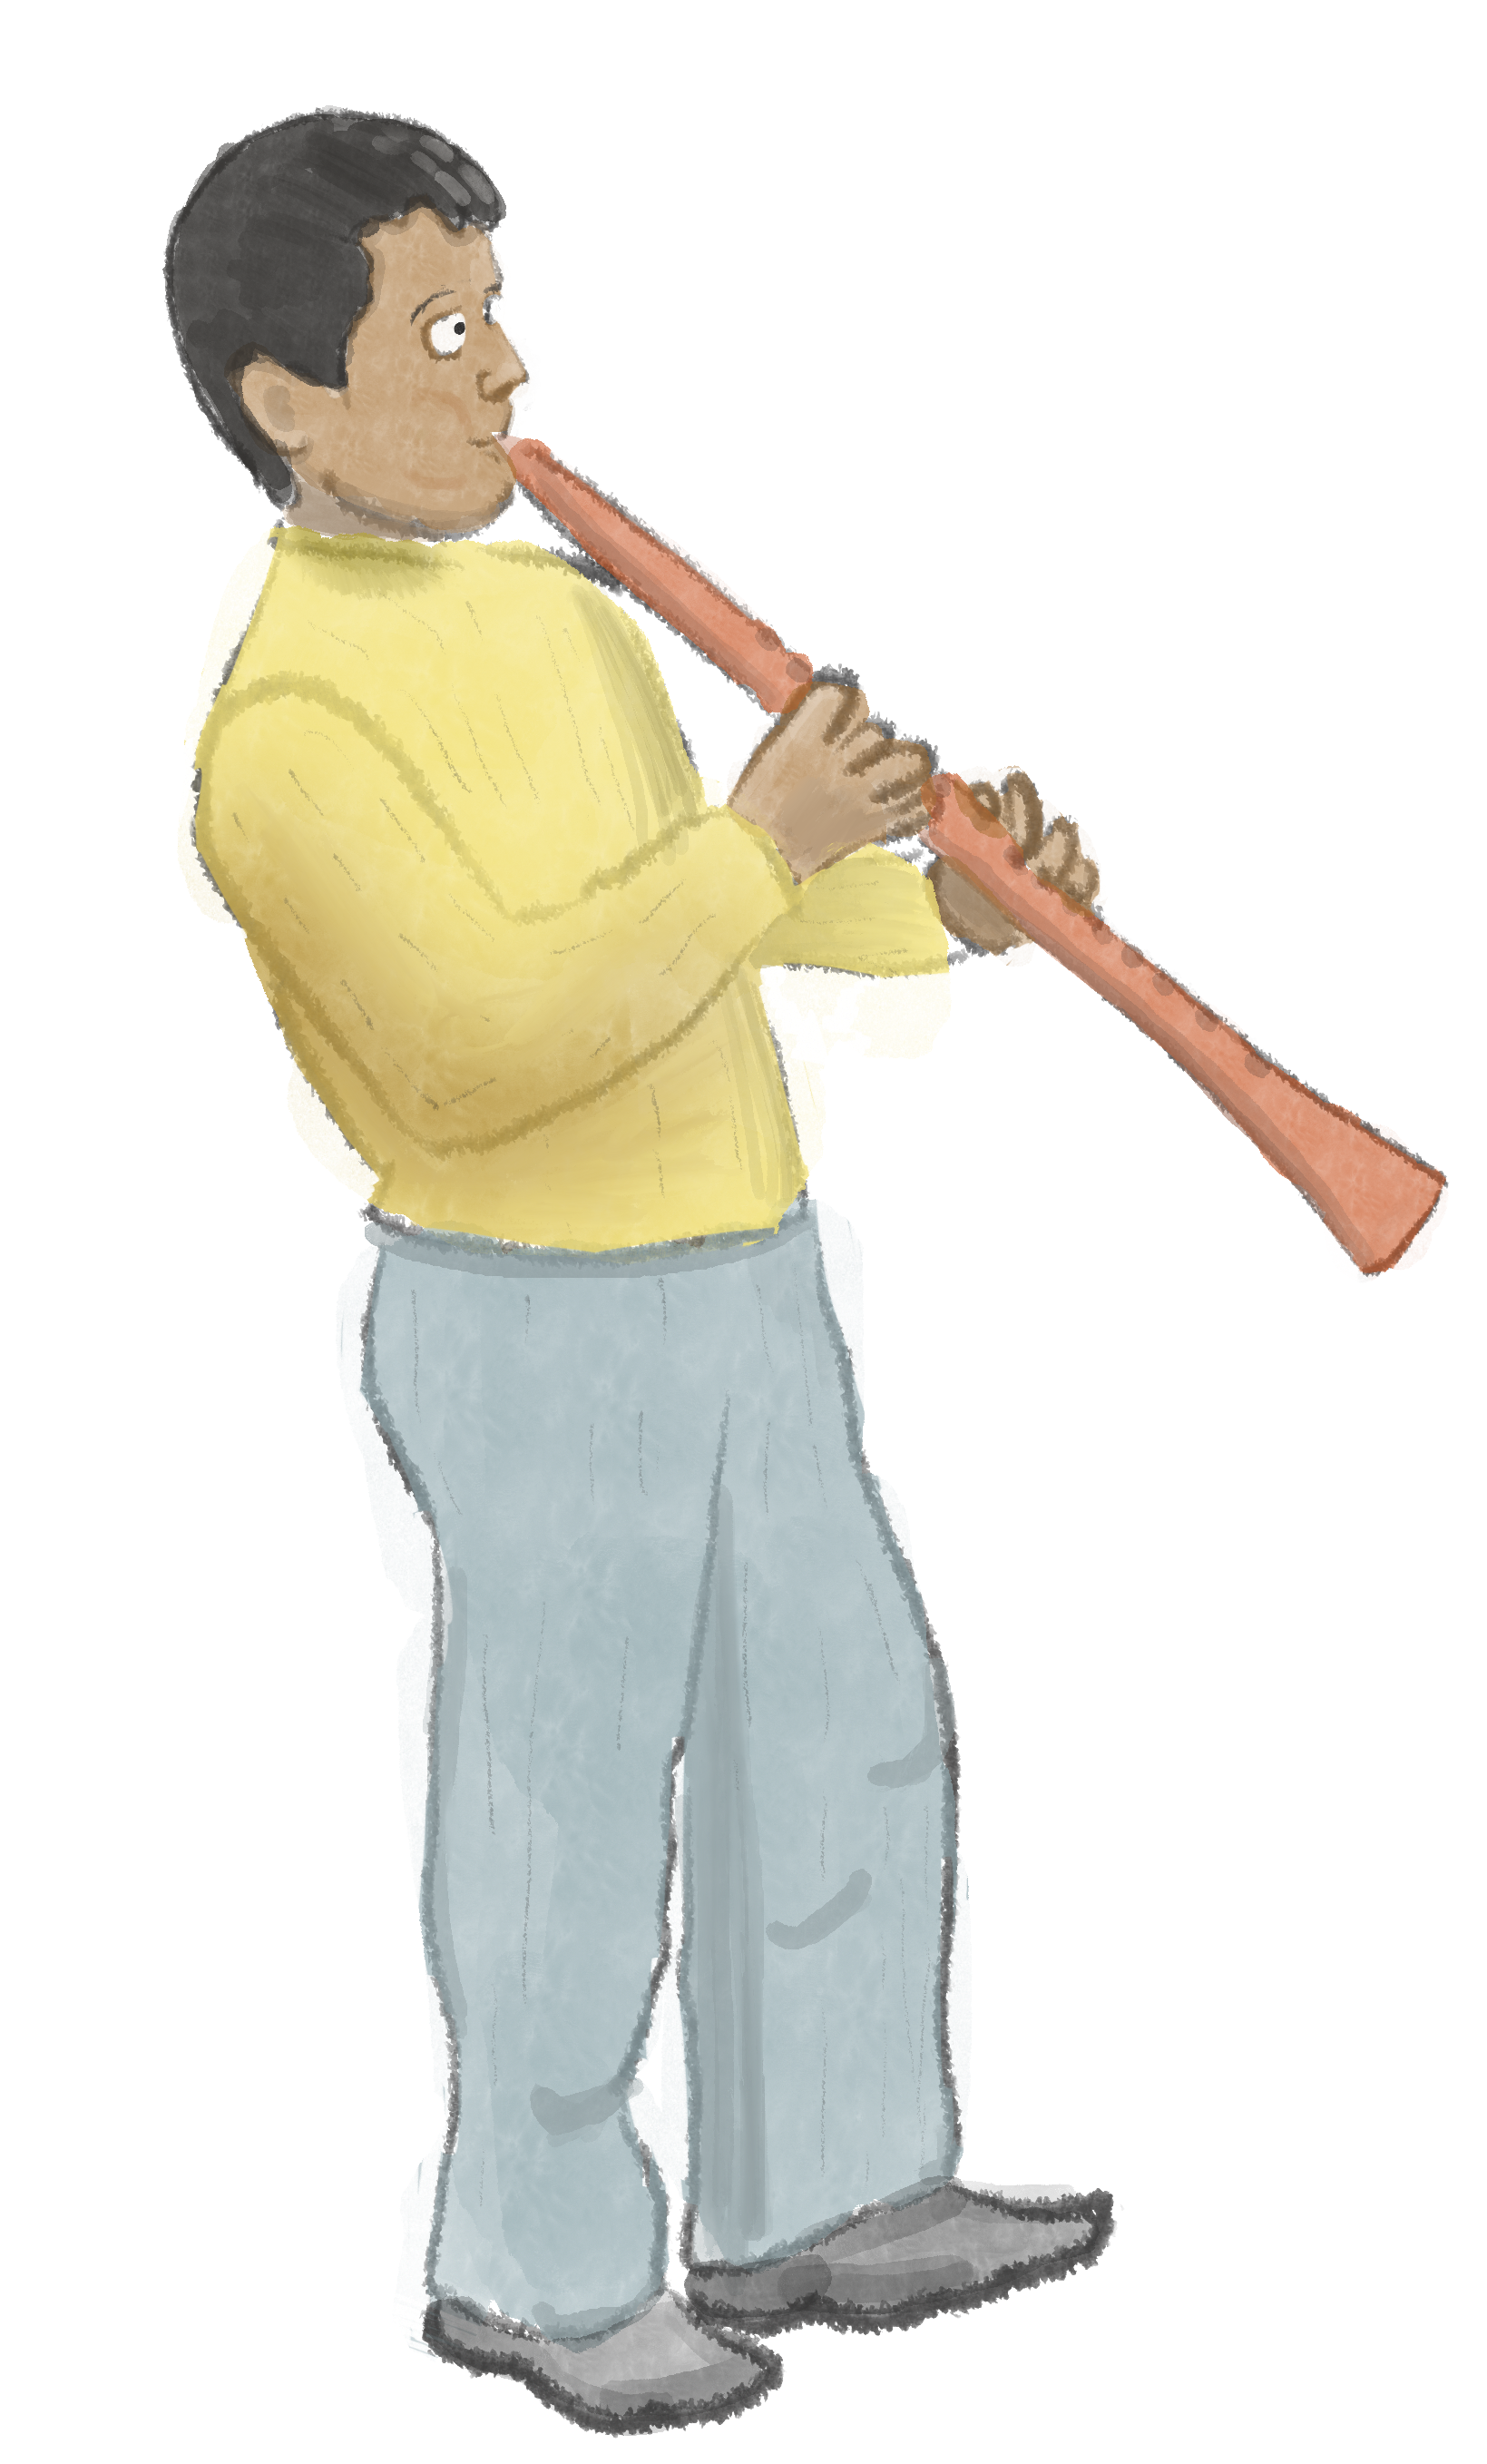
\includegraphics[width=7.0cm]{boy.png}} % Adjust the coordinates and size as needed
}
\end{document}
